\chapter{Аналитический раздел}
В данном разделе будет проведен анализ предметной области с целью выявления особенностей дискретно-событийного моделирования и распределения событий в реальных системах массового обслуживания. Будут проанализированы существующие алгоритмы продвижения модельного времени, а также формализована постановка задачи в виде IDEF0-диаграммы.

\section{Анализ предметной области}
Многие задачи дискретно-событийного моделирования тесно связаны с теорией
массового обслуживания \cite{imitation_modelling_def}. Объектом изучения теории массового обслуживания (ТМО) являются системы массового обслуживания (СМО). В настоящее время разработано множество математических моделей, позволяющих изучать совершенно различные реально протекающие процессы обслуживания в сфере транспорта, в промышленном производстве, образовании, медицине, военном деле, торговле, телефонии, компьютерных сетях и т.д \cite{gpss}. Модель представляет собой абстрактное описание системы, уровень детализации которой зависит от цели моделирования и возможности получения исходных данных с необходимой точностью \cite{mass_service_systems}. Конечная цель развиваемых в ТМО методов состоит в поиске рациональной структуры обслуживающей системы и ее параметров, а также организации обслуживания, обеспечивающей необходимое его качество.

Под системой массового обслуживания понимают системы, производящие обслуживание поступающих в нее запросов на выполнение каких-либо услуг. Каждая СМО состоит из некоторого числа обслуживающих устройств --- каналов (приборов) обслуживания.
На вход СМО поступает один или несколько потоков запросов (заявок), требующих однотипного обслуживания. К основным элементам СМО относят:
\begin{itemize}
	\item входящий поток заявок;
	\item очередь;
	\item каналы обслуживания;
	\item выходящий поток обслуженных заявок.	
\end{itemize}

Для описания системы массового обслуживания необходимо задать вероятностные законы, определяющие последовательность моментов поступления заявок в систему и продолжительность обслуживания, а также принцип, в соответствии с которым поступающие в систему заявки выбираются из очереди на обслуживание (FIFO, LIFO, случайный отбор и т.д.).

Системы массового обслуживания можно классифицировать по следующим признакам:
\begin{enumerate}
	\item По числу фаз обслуживания --- \textit{однофазные} и \textit{многофазные}.
	\item По числу каналов --- \textit{одноканальные} и \textit{многоканальные}. Многоканальные СМО, в свою очередь, могут подразделяться на \textit{полнодоступные}, подразумевающие однородные каналы (с одинаковыми характеристиками), и \textit{неполнодоступные}, соответственно, с различными характеристиками каналов.
	\item По вероятностным характеристикам времени обслуживания --- \textit{со случайным временем обслуживания} и \textit{с фиксированным постоянным временем обслуживания}.
	\item По характеру случайного процесса, происходящего в СМО --- \textit{маркковские} и \textit{немарковские}. Случайный процесс называется марковским, если для каждого момента времени вероятность любого состояния системы в будущем зависит только от ее состояния в настоящем и не зависит от того, когда и каким образом система пришла в это состояние, т.е. не зависит от того, как процесс развивался в прошлом. Для марковской СМО легко описать математическую модель, однако в реальной жизни таких систем не бывает. Немарковские системы требуют применения статистического моделирования с использованием ЭВМ.
	\item По наличию возможности ожидания обслуживания  --- \textit{с отказами} и \textit{с ожиданием}. В системах с отказами заявка, поступившая в момент, когда все каналы заняты, получает отказ и покидает систему. В системах с ожиданием при занятости всех каналов обслуживания заявка становится в очередь и ждет освобождения одного из каналов. СМО с ожиданием, в свою очередь, можно разделиь на системы \textit{с ограниченным} (по длине очереди или по времени ожидания в очереди) и \textit{неограниченным} ожиданием.
	\item По наличию приоритетов обслуживания --- \textit{без приоритетов} и \textit{с приоритетами}.
	\item По наличию ограничений, накладываемых на поток заявок, --- \textit{замкнутые}, подразумевающие ограниченный поток заявок, которые после обслуживания могут возвращаться в СМО, и \textit{открытые}.
\end{enumerate}


Как уже было сказано ранее, системы массового обслуживания оперируют понятием заявки. Такие события, как поступление новой заявки, начало ее обслуживания и т.д. вызывают изменение состояния системы и образуют \textit{поток событий} --- последовательность однородных событий, следующих одно за другим через некоторые интервалы времени. Такой поток обладает свойством дискретности и носит стохастический характер функционирования ввиду того, что момент попадания новой заявки и время ее обслуживания случайны.

%Период от момента поступления заявки в СМО и до начала обслуживания называется \textit{временем ожидания обслуживания}. Время ожидания обслуживания в совокупности с временем обслуживания составляет \textit{время пребывания требования в системе}.


Для имитацию параллельных событий, происходящих в реальной системе, вводят некоторую глобальную переменную, обеспечивающую синхронизацию всех событий в системе, которую называют модельным (или системным) временем. Для того, чтобы вести отсчет модельного времени и обеспечить правильную хронологическую последовательность наступления основных событий в имитационной модели, используется так называемый таймер модельного времени, который представляет собой переменную для хранения текущего значения модельного времени.

В процессе моделирования системы таймер модельного времени должен постоянно корректироваться в соответствии с основными событиями, возникающими в реальной системе, поэтому одной из важнейших задач имитационного моделирования является \textbf{продвижение модельного времени}.

При рассмотрении реальных СМО можно заметить, что распределение событий в них отнюдь не однородно: события группируются вдоль временной оси \cite{system_modelling}. Начало возникновения групп связано с наступлением некоторого события или их множества. Такой момент времени называется \textit{синхронным моментом}, а наступившее в этот момент событие --- \textit{событием синхронизации}. Интервал, следующий за синхронным моментом времени, обладает плотностью событий, значительно выше средней, и называется \textit{пиковым интервалом}. Причиной появления пиковых интервалов является наличие в системе особых событий, возникновение которых порождает другие события. В качестве примера можно привести синхронизирующие сигналы, переключающие множество триггеров в цифровых сетях.

Рассмотрим временную ось, представленную на рисунке \ref{img:delft_example}. Интервалы вида $[t_i, t_i + t_p]$ $(i = 1, 2, ...)$ являются пиковыми, а точки $t_i$ $(i = 1, 2, ...)$ представляют собой синхронные моменты времени.

\begin{figure}[h!btp]
	\centering
	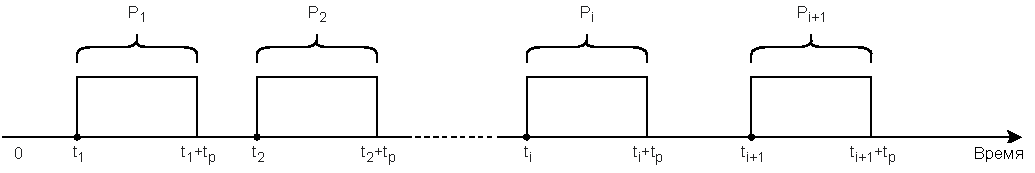
\includegraphics[width=0.9\columnwidth]{inc/img/delft_example.pdf}
	\caption{Квазисинхронное распределение событий}
	\label{img:delft_example}	
\end{figure}

\textit{Квазисинхронным (пиковым) распределением} событий называется распределение, при котором значение $p$ вероятности возникновения события значительно больше в интервалах времени $[t_i, t_i + t_p]$, чем в промежуточных интервалах $[t_i + t_p, t_{i+1}]$ $(i = 1, 2, ...)$, при $t_{i+1} - t_i > t_p$.

В рассматриваемом случае допускается одновременное возникновение нескольких событий. Также не исключается возможность того, $t_{i+1} - t_i < t_p$ при $t_i \neq i \cdot t_1$.


Алгоритмы продвижения модельного времени должны быть адаптированы под моделирование систем, распределение событий в которых является пиковым.

\section{Алгоритмы продвижения модельного времени}

\subsection{Пошаговый алгоритм}
Данный алгоритм подразумевает продвижение модельного времени на фиксированное $\delta t$ единиц. После каждого обновления часов проверяется, произошли ли какие-либо события в течение предыдущего интервала времени $\delta t$. Если на этот интервал запланировано одно или несколько событий, считается, что данные события происходят в конце интервала, после чего состояние системы и счетчики обновляются соответствующим образом. 

Продвижение времени посредством пошагового алгоритма представлено на рисунке \ref{img:delta_t_example}.

\begin{figure}[h!btp]
	\centering
	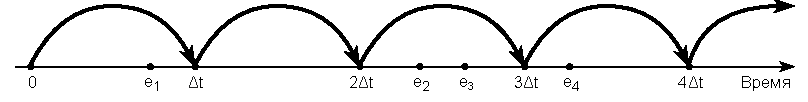
\includegraphics[width=0.7\columnwidth]{inc/img/delta_t_example.pdf}
	\caption{Пример продвижения времени посредством пошагового алгоритма}
	\label{img:delta_t_example}	
\end{figure}

Изогнутыми стрелками обозначено продвижение часов модельного времени, а $e_i$ $(i = 1, 2, ...)$ --- это реальное время возникновения события $i$ любого типа.

Рассмотрим несколько представленных интервалов:
\begin{itemize}
	\item в интервале $[0, \delta t)$ событие происходит в момент времени $\delta t$;
	\item в интервале $[\delta t, 2\delta t)$ не происходит ни одного события, однако проверка на наличие событий все равно выполняется;
	\item в интервале $[2\delta t, 3\delta t)$ события происходят в моменты времени $e_2$, $e_3$, однако считается, что они произошли в момент времени $3\delta t$.
\end{itemize}

Заметим, что возникает сложность обработки событий, произошедших в один и тот же временной интервал. Данную проблему можно решить уменьшением размера интервала, однако в таком случае возрастает число проверок возникновения событий, что приводит к значительному увеличению времени выполнения программы. 

Ввиду этой особенности продвижение модельного времени с помощью пошагового алгоритма не используется в тех случаях, когда интервалы времени между последовательными событиями слишком отличны по своей продолжительности \cite{imitation_modelling}. 

Таким образом, продвижение времени посредством постоянного шага имеет два недостатка:
\begin{itemize}
	\item сложность обработки событий, рассматриваемых как одновременные, однако в действительности произошедших в разное время;
	\item  значительные затраты вычислительных ресурсов.
\end{itemize}

В основном этот алгоритм используется для моделирования систем, в которых можно допустить, что все события в действительности происходят в один из моментов $n$ времени $\delta t$ $(n = 0, 1, 2, ...)$ для соответственно выбранного $\delta t$ \cite{imitation_modelling}. 

\subsection{Событийный алгоритм}
При использовании данного алгоритма продвижение модельного времени происходит в моменты возникновения событий в системе.
Предварительно определяется время возникновения будущих событий, после чего таймер модельного времени принимает значение, равное времени возникновения ближайшего события, и в этот момент обновляется состояние системы с учетом произошедшего события, а также сведения о времени  возникновения будущих событий. Затем значение таймера модельного времени продвигается ко времени возникновения нового ближайшего события, аналогично обновляется состояние системы и определяется время будущих событий, и т. д.

Процесс продвижения модельного времени от времени возникновения одного события ко времени возникновения другого продолжается до тех пор, пока не будет выполнено какое-либо заранее установленное условие останова. Поскольку в дискретно-событийной имитационной модели все изменения происходят только во время возникновения событий, периоды бездействия системы просто пропускаются, и часы модельного времени переводятся со времени возникновения одного события на время возникновения другого. При таком подходе длительность интервала продвижения модельного времени от одного события к другому может быть различной.

На рисунке \ref{img:delta_z_example} представлен механизм продвижения модельного времени в системе массового обслуживания с одним устройством обслуживания.

\begin{figure}[h!btp]
	\centering
	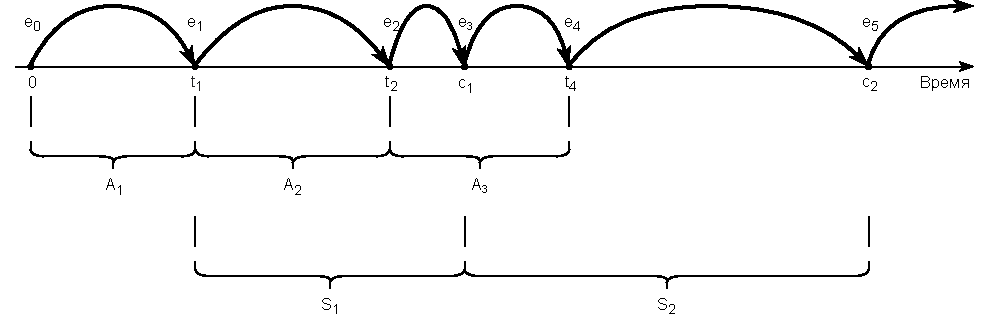
\includegraphics[width=0.8\columnwidth]{inc/img/delta_z_example.pdf}
	\caption{Пример продвижения времени посредством событийного алгоритма}
	\label{img:delta_z_example}	
\end{figure}

Рассмотрим следующие обозначения:
\begin{itemize}
	\item $t_i$ --- время поступления $i$-й заявки ($t_0 = 0$);
	\item $A_i = t_i - t_{i-1}$ --- время между поступлением заявок $i-1$ и $i$; 
	\item $S_i$ --- время, потраченное устройством на обслуживание требования $i$ (без учета времени задержки заявки в очереди);
	\item $D_i$ --- время задержки $i$-й заявки в очереди;
	\item $c_i = t_i + D_i + S_i$ --- время ухода $i$-й заявки по окончании обслуживания;
	\item $e_i$ --- время возникновения события $i$ любого типа.
\end{itemize}

Допустим, известны законы распределения вероятностей для времени между поступлением заявок $A_i$ и $A_{i+1}$ и для времени обслуживания $S_i$, заданные функциями распределения $F_A$ и $F_S$ соответственно. Тогда значения $A_i$ будут генерироваться на основе $F_A$, а $S_i$ --- на основе $F_S$.
В момент времени $e_0 = 0$ обработчик заявок незанят. После генерации времени поступления первой заявки $A_1$ таймер модельного времени принимает значение времени возникновения следующего (первого) события $e_1 = t_1$. Ввиду того, что в момент поступления в систему первой заявки обработчик заявок незанят, он немедленно начинает обслуживание с задержкой заявки в очереди $D_1 = 0$, изменяя свое состояние на занятое. Время окончания обслуживания заявки $c_1$ вычисляется путем прибавления сгенерированного $S_1$ к $t_1$. 

Время поступления в систему второй заявки $t_2$ определяется по формуле $t_2 = t_1 + A_2$. Если $t_2 < c_1$, как показано на рисунке \ref{img:delta_z_example}, таймер модельного времени принимает значение времени возникновения следующего события $e_2 = t_2$, иначе --- значение окончания обслуживания первой заявки $c_1$. Так как в момент времени поступления новой заявки $t_2$ обработчик заявок находится в состоянии обслуживания предыдущей заявки (занят), число заявок в очереди увеличивается с 0 до 1. В таком случае сохраняется время поступления заявки, однако не генерируется время обслуживания $S_2$. 

Время поступления в систему третьей заявки вычисляется по формуле $t_3 = t_2 + A_3$. Если $с_1 < t_3$, таймер модельного времени принимает значение времени возникновения следующего события $e_3 = c_1$. Когда заявка, обслуживание которой завершено, покидает систему, начинается обслуживание заявки в очереди, при этом длина очереди уменьшается на 1. Время задержки взятой из очереди заявки вычисляется по формуле $D_2 = c_1 - t_2$, а время окончания обслуживания обработчиком --- $c_2 = c_1 + S_2$. Аналогично если $t_3 < c_2$, таймер модельного времени принимает значение времени возникновения следующего события $e_4 = t_3$ и т.д. 

Моделирование может быть завершено, например, по окончании обслуживания заданного числа заявок или по истечении заданного максимального времени моделирования.


Данный алгоритм целесообразно использовать при моделировании систем, в которых события распределены во времени неравномерно или в тех случаях, когда необходимо точное определение или квазипараллельная обработка одновременных событий \cite{imitation_modelling}.

\section{Оценка сложности алгоритмов}
Сложность рассмотренных алгоритмов в общем зависит от вида распределения событий в моделируемой системе, от их количества, а также от общего времени моделирования.
Заметим, что сложность пошагового алгоритма также зависит от количества блоков, генерирующих события в системе, т.к. при каждом тике времени происходит полный обход всех блоков системы для проверки наличия нового события.

\subsection{Пошаговый алгоритм}
Приняв минимальный тик таймера модельного за времени за единицу, будем считать, что пошаговый алгоритм, используя это значение в качестве $\Delta t$, исключает возможность пропуска событий.

Оценка алгоритмической сложности пошагового алгоритма продвижения модельного времени зависит от количества операций, которые необходимо выполнить при каждом тике таймера модельного времени. Для системы с множеством блоков сложность может быть оценена как $O(N*M)$, где $N$ --- общее время моделирования, выраженное в тиках таймера, а $M$ --- количество операций, необходимых для обработки каждого тика (пропорционально количеству блоков, генерирующих события в моделируемой системе).

\subsection{Событийный алгоритм}
Событийный алгоритм представляет собой обход сортированного списка (очереди с приоритетом) с последующим добавлением в этот же список (очередь) новых событий. Приоритет событий в очереди определяется временем возникновения события в системе.
В худшем случае при обработке одного события в очередь будут добавлены два новых события --- событие об окончании генерации новой заявки и событие об окончании обработки заявки. Для оценки сложности алгоритма необходимо учесть сложность операций вставки и получения элемента в очередь с приоритетом.


Алгоритмическая сложность вставки элемента в очередь с приоритетом зависит от реализации очереди. Наиболее распространенная реализация очереди с приоритетом  --- куча (heap) \cite{priority_queue_implementation}. Сложность операции вставки элемента в такую очередь с приоритетом составляет $O(log N)$, где $N$ - количество элементов в очереди \cite{priority_queue_complexity}. При использовании других реализаций (например, на основе бинарного или сбалансированного дерева), сложность операции вставки элемента может быть другой, однако не хуже приведенной выше  \cite{priority_queue_implementation}.


Сложность получения элемента из очереди с приоритетом имеет алгоритмическую сложность $O(1)$, ввиду того, что корень кучи всегда содержит элемент с наивысшим приоритетом \cite{priority_queue_implementation}.
В других реализациях очереди с приоритетом сложность операции получения элемента может быть выше, например, $O(\log{N})$, где $N$ --- количество элементов в очереди \cite{priority_queue_implementation}. Это связано с тем, что при поиске элемента с наивысшим приоритетом может потребоваться пройти по дереву от корня до листа, что занимает логарифмическое время.
В данной работе рассматривается событийный алгоритм, использующий для списка будущих событий очередь с приоритетом, основанную на куче, ввиду чего сложность операций вставки и получения события составляет соответственно $O(\log{N})$ и $O(1)$.


Тогда оценка алгоритмической сложности событийного алгоритма продвижения модельного времени зависит от общего количества обрабатываемых событий и, с учетом рассмотренной выше реализации, может быть оценена как $O(N\log{N})$, где $N$ --- количество событий, обрабатываемых за указанное время моделирования.

\subsection{Выводы}
На основе приведенной оценки сложности алгоритмов можно сделать вывод о том, что временная эффективность алгоритмов стремительно падает в случае пикового распределения событий в моделируемой системе. Падение эффективности тем больше, чем большее количество блоков, генерирующих события, содержит система.
Пошаговый алгоритм становится тем неэффективнее, чем больше длина временных промежутков между пиковыми интервалами, ввиду невозможности пропустить временные промежутки, не содержащие событий. Событийный же алгоритм стремительно теряет эффективность из-за высокой плотности событий на пиковых интервалах, ввиду роста сложности вставки событий в список будущих событий.

\section{Постановка задачи}
Таким образом, необходимо разработать алгоритм, рассчитанный на моделирование сложных систем (состоящих из большого числа блоков), распределение событий в которых является пиковым. Алгоритм, комбинирующий в себе особенности пошагового и событийного алгоритма, должен решить проблемы падения временной эффективности по причинам, приведенным в предыдущем пункте.

IDEF0-диаграмма для комбинированного алгоритма продвижения модельного времени представлена на рисунках \ref{img:IDEF0-A0} \ref{img:IDEF0-A1}.

\begin{figure}[h!btp]
	\centering
	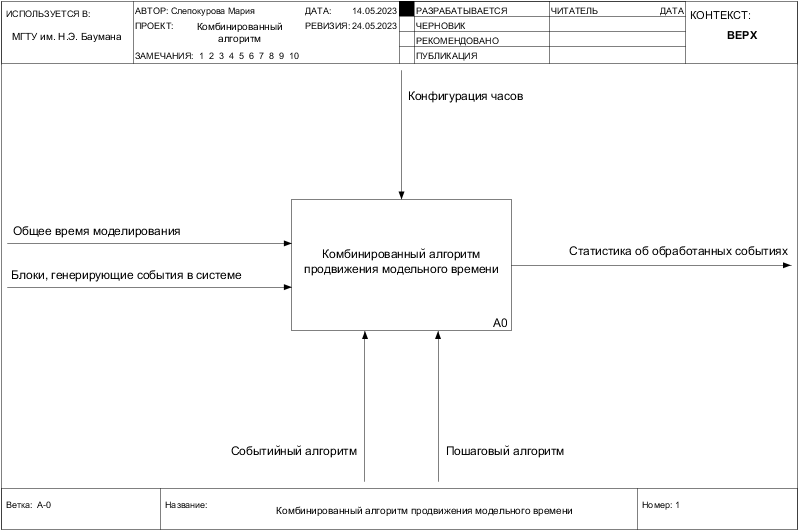
\includegraphics[width=1\columnwidth]{inc/img/IDEF0-A0.png}
	\caption{IDEF0 нулевого уровня}
	\label{img:IDEF0-A0}	
\end{figure}

\begin{figure}[h!btp]
	\centering
	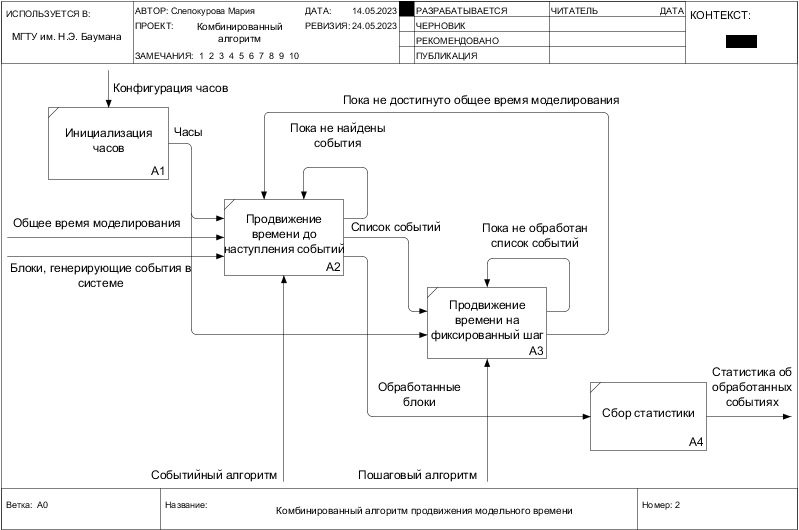
\includegraphics[width=1\columnwidth]{inc/img/IDEF0-A1.png}
	\caption{IDEF0 первого уровня}
	\label{img:IDEF0-A1}	
\end{figure}

\section{Выводы}
В рамках данного раздела были рассмотрены существующие алгоритмы продвижения модельного времени. Была проведена оценка сложности рассмотренных алгоритмов, а также выявлены их недостатки в контексте проанализированной предметной области. На основе полученных заключений была сформулирована цель данной работы, а также формализована постановка задачи в виде IDEF0-диаграммы.
